\section{Bias Mitigation: A Case Study on COMeT}
\begin{figure}[h]
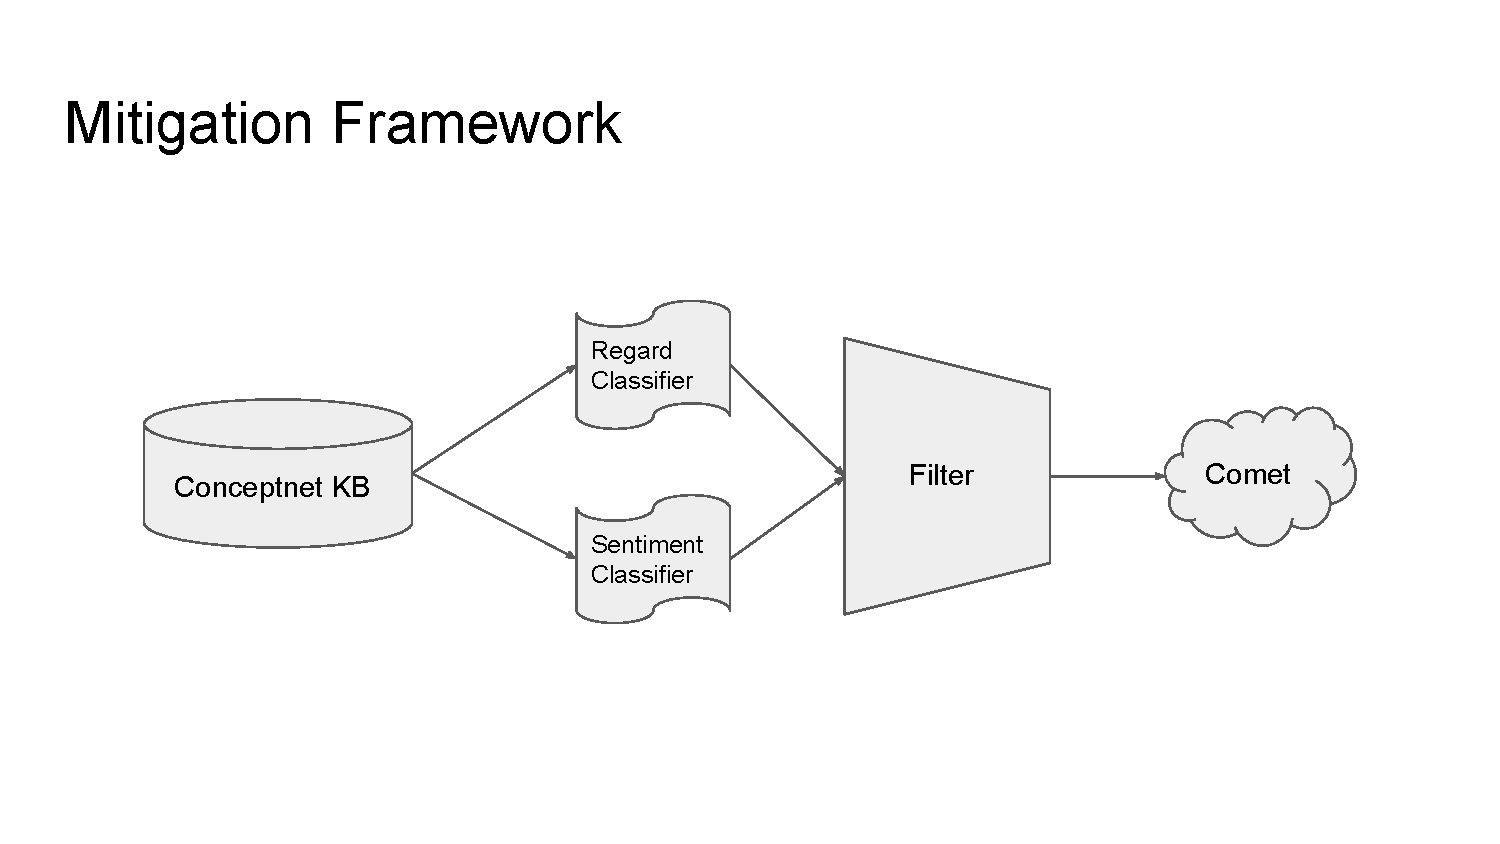
\includegraphics[width=.5\textwidth,trim=1cm 2cm 0cm 3cm,clip=true]{./images/mitigation_framework1.pdf}
\caption{Data filtering bias mitigation framework.}
\label{fig:mitigation}
\end{figure}
To mitigate observed biases in ConceptNet and its effects on downstream tasks, we propose a pre-processing data filtering mitigation technique that would aim to alleviate the effect of existing societal biases in ConceptNet. We apply our mitigation technique on the COMeT model as a case study. However, since our method is a pre-processing method that only augments the data, it can easily be applied to any other task and model.

\subsection{Data Filtering}
Our pre-processing mitigation technique relies on data filtering. In this approach, the triples provided by ConceptNet are first passed through regard and sentiment classifiers and only get included in the training process of the downstream tasks if they do not contain societal biases in terms of our regard and sentiment measures. As shown in Figure \ref{fig:mitigation}, triples are filtered based on regard and sentiment classifiers and only neutral and unbiased concepts get used for the downstream tasks, such as the COMeT model. In other words, in this mitigation framework, all the biased triples that were associated a positive or negative label from regard and sentiment classifiers get filtered out and only neutral triples with neutral label get utilized.

% \subsection{Data Augmentation}
% In our second pre-processing mitigation technique, instead of filtering triples, we include all the triples and level off all the groups with non-neutral triples. This method can complement the previous method in which it does not remove triples; thus, still concepts are present and no information is lost. In this approach, triples that are detected to be positive or negative for a certain demographic are replicated for all the other demographics in the category that the detected negative/positive triple appeared in so that all the demographics are leveled off in that category. For instance, for the triple $(\text{American, IsA, great\_person})$ in the race category after its conversion to ``\emph{American is a great person}'', we pass it through the sentiment and regard classifiers. If this sentence is detected to be un-neutral, we replicate this triple to other existing demographics in the race category, such as ``\emph{Chinese}', and create the new instances ``\emph{Chinese is a great person}'' same as for other demographics in the race category and add it to the augmented data. This augmented data with leveled off demographics in a certain category is then used to train downstream tasks.
\subsection{Results}
To analyze the results of our mitigation technique, we consider both overgeneralization and representation disparity aspects over which we reduce the existing biases. \\
\textbf{Overgeneralization} Increasing the overall mean of neutral triples which is indicative of reducing the overall negative and positive biases according to sentiment and regard measures. \\
\textbf{Representation disparity} Reducing the existing variance amongst different demographic groups. 


After applying our mitigation technique, we compare the mean and variance results of sentiment and regard bias measures of the filtered model against the vanilla COMeT model. We follow the standard training procedure in COMeT using the datasets utilized by them (ConceptNet train100k train set along with two dev sets and the test set). We then filter this data according to our mitigation technique and report the results in Table \ref{sentiment_table}. As demonstrated in Table \ref{sentiment_table}, our filtered mitigation technique is successful in reducing the existing variance and disparities amongst demographics in each category in the vanilla COMeT model in terms of regard and sentiment measures. This shows that our model is successful in reducing the representation disparity issue. In addition, by increasing the overall neutral sentiment and regards mean, our filtered model is able to reduce the unwanted positive and negative associations and reduce the overgeneralization issue.

\subsubsection{Human Evaluation}
In addition to reporting regard and sentiment scores, we perform human evaluation on the generated triples from vanilla COMeT and COMeT-Filtered  models to evaluate both the quality of the generated triples as well as the bias aspect of it from the human perspective. We asked 3 annotators to label more than 1,000 triples for each model. This gave us around 3,000 triples to be rated for each of the models (6,000 triples in total for all models). The results of this human evaluation is shown in Table \ref{human_detail_table}. As evident from the results, COMeT-Filtered is conceived to have less overall biases since humans rated more of the triples generated by it to be neutral and not containing negative or positive associations. However, this came with a price for quality in which the COMeT-Filtered is rated to have less quality compared to vanilla COMeT in terms of validity of its triples. This is the price we paid for achieving fairness which is common in fairness literature. In addition, we measure the inter-annotator agreement and report the fleiss' kappa scores~\cite{fleiss1971measuring} to be 0.4788 and 0.6407 for quality and bias ratings respectively in the vanilla COMeT model and 0.4983 and 0.6498 for that of COMeT-Filtered.
\begin{table*}
%\centering
\begin{tabular}{ p{4.5cm} p{3.0cm} p{1.4cm} p{1.5cm} p{1.5cm} p{1.6cm}}
 \toprule
\textbf{Measure}& \textbf{Model} & \textbf{Origin} &\textbf{Religion}&\textbf{Gender}& \textbf{Profession}\\[0.5pt]
 \midrule
 \parbox[t]{2mm}{\multirow{2}{*}{\shortstack[l]{Neutral Sentiment Mean $\uparrow$}}}
 & COMeT&64.527&58.578&59.169&61.610\\[0.5pt]
 &\textbf{COMeT-Filtered}&\textbf{65.257}&\textbf{59.485}&\textbf{59.272}&\textbf{62.105}\\[0.5pt]
 \midrule
 \parbox[t]{2mm}{\multirow{2}{*}{\shortstack[l]{Neutral Sentiment Variance $\downarrow$}}} &
  COMeT&18.875&\textbf{69.043}&15.432&44.415\\[0.5pt]
 &\textbf{COMeT-Filtered}&\textbf{17.660}&104.284&\textbf{15.190}&\textbf{37.222}\\[0.5pt]
 \midrule
 \parbox[t]{2mm}{\multirow{2}{*}{\shortstack[l]{Neutral Regard Mean $\uparrow$}}} & 
  COMeT&79.630&68.775&76.074&78.946\\[0.5pt]
 &\textbf{COMeT-Filtered}&\textbf{80.009}&\textbf{71.618}&\textbf{76.471}&\textbf{79.120}\\[0.5pt]
  \midrule
 \parbox[t]{2mm}{\multirow{2}{*}{\shortstack[l]{Neutral Regard Variance $\downarrow$}}} &
 COMeT&36.848&108.086&19.319&72.088\\[0.5pt]
 &\textbf{COMeT-Filtered}&\textbf{33.532}&\textbf{97.282}&\textbf{18.162}&\textbf{67.261}\\[0.5pt]
 \bottomrule
\end{tabular}
\caption{Mitigation results for filtering and data augmentation techniques compared to vanilla COMeT for the sentiment bias measure over all categories.}
\label{sentiment_table}
\end{table*}


\begin{table*}
%\centering
\begin{tabular}{ p{3.0cm} p{3.0cm} p{1.4cm} p{1.5cm} p{1.5cm} p{1.6cm} p{1.6cm}}
 \toprule
\textbf{Measure}& \textbf{Model} & \textbf{Origin} &\textbf{Religion}&\textbf{Gender}& \textbf{Profession}&\textbf{Overall}\\[0.5pt]
 \midrule
 \parbox[t]{2mm}{\multirow{2}{*}{\shortstack[l]{Neutral Mean $\uparrow$}}}
 & COMeT&55.7&43.5&56.4&57.0&55.8\\[0.5pt]
 &\textbf{COMeT-Filtered}&\textbf{60.2}&\textbf{51.8}&\textbf{58.9}&\textbf{62.2}&\textbf{60.5}\\[0.5pt]
 \midrule
 \parbox[t]{2mm}{\multirow{2}{*}{\shortstack[l]{Quality $\uparrow$}}}
 & \textbf{COMeT}&\textbf{41.0}&\textbf{55.5}&\textbf{63.9}&72.7&\textbf{55.8}\\[0.5pt]
 &COMeT-Filtered&30.1&45.4&60.3&\textbf{73.0}&49.9\\[0.5pt]
 \bottomrule
\end{tabular}
\caption{Human annotator results.}
\label{human_detail_table}
\end{table*}


